\chapter{Case Study: JUNE}
% \setcounter{section}{0}
\label{chapter:june}
\textbf{CURRENTLY IN MARKDOWN, JUST FIX!}

This document is not a finalised profile report for a JUNE, more a set of notes
as to how I have gone about profiling JUNE's performance.

\section{Getting started}
Firstly, we download JUNE's source code onto a cluster and build the JUNE
Python package. This is all well documented elsewhere and principally just
relies on a recent version of Python (typically from v3.12) and an OpenMPI
installation.

Secondly, once installed we need to understand the very basic workflow of the
JUNE code. There are essentially two main steps:
\begin{enumerate}
    \item Generate the world, including the population and geography - \\
   \verb|example_scripts/create_world.py|
   \item Run the simulation of a disease spreading throughout this population - \\
   \verb|example_scripts/run_simulation.py|
\end{enumerate}
 
Step 1. creates an output file \verb|tests.hdf5| which contains data on the world
population. This data has to be fed into the \verb|run_simulation.py| script which
then goes through two routines: (a) load in population/geography data; (b)
restore population/geography objects.

Thirdly, we need to understand at a very basic level the way we run this
workflow, e.g., the \verb|create_world.py| runs in serial. Seems as though this has
never been parallelised for the pragmatic reason that this script only really
needs to be generated once as this the 'world' only needs to be generated once
per scenario (e.g., England, London, etc.). Therefore, the 'developer' time can
be saved because the \verb|create_world.py| script may take a long time but it is
run infrequently. On the other hand, the \verb|run_simulation.py| script comes with
MPI functionality and so we need to keep this in mind that this is our only
resource variable.

Fourthly, before running any job scripts we want to understand what we are
going to run. There are two primary simulations that JUNE is equipped for
(though is now greater functionality), which are:
* London - along with some other msoas in the South of England
* England - the total population run of England
 The England simulation is by definition the most demanding and is therefore:
'what we are aiming for'.  However, when trying to get an understanding of the
resources, scaling and access patterns of a code, it is useful to start with a
simpler, or test, case.  Hence, we begin with the London case. Once we have
gained an understanding of this smaller case, it may be useful to understand
how the problem scale impacts performance.

\section{Basic metrics}
I want to know, for a serial run, the runtime and memory usage of both the
\verb|create_world.py| and \verb|run_simulation.py| scripts, as this is our basic
starting point of performance. This is our starting point to really coarsely
understand what we are working with.

To do this we simply use SLURM's accounting command
\begin{verbatim}
sacct -j <job-id> -o maxRSS,elapsed
\end{verbatim}
i.e., for a specific job this gives us:
\begin{itemize}
    \item \verb|maxRSS| - the maximum memory consumption seen by one of the tasks
    \item \verb|elapsed| - the total elapsed runtime
\end{itemize}
This is useful as it gives us the base line performance we are working with.
Similarly it is very useful to know the maximum memory consumption as this may
have implications on the hardware availability and decision. We claim that our
'test case' has a runtime small enough such that this is not of major concern
(e.g., max of say around 30 minutes). However, memory consumption may be
significant and it useful to consult the hardware documentation of a cluster to
know how close to a node maximum memory the job is. In a case of significant
memory usage - relative to the available memory - then it is useful to note
that this may play a role in node scaling.

\subsection{England resources}
For this particular code, the 'typical full simulation size' is well known, as
it is a simulation of the total England population. Our thought here is that
this is not a simple problem scaling to go from London to England, i.e., this
is not as simple as doubling a quantity of grid points. Hence, we run a serial
version of \verb|create_world.py| and \verb|run_simulation.py| for the total of England
also, as we want to get an idea of how this problem scales, and again if there
are concerns for memory usage.

This is not necessary for all performance analysis, i.e., it may be overkill to
analyse a test case and a 'full' case for each code base. However, because we
know concretely what the 'full case' is, then we perform a simple resource
metric output for this case along side the London 'test' case. We can then use
the output of memory and runtime to understand how the problem itself scales,
e.g., London has a population of approximately one sixth of England, and so if
the problem scaled linearly we would see approximately a six times increase in
runtime and memory. The agents within JUNE have quite complex structures of
friendships and sexual networks, hence these data structures would be predicted
to not scale linearly which again could impact how we perform our performance
analysis. 

\textbf{Checkpoint:} This can be a useful point to go back to the researcher and
discuss the problem scaling and resources used. For example, the resources used
may not be of direct interest to the researcher, but the problem scaling is
likely a result of the algorithm used and they may have input to say that this
is not scaling as predicted, which can again point you towards
performance/scaling issues.

\section{Profile}
\emph{Bare bones scaling, e.g., gprof}
Understanding the basic resource use of a code is very beneficial. To go one
step beyond the basic resource usage, this profile should give function
runtimes, i.e., something like a flame or icicle graph. These plots often give
graphical representations of similar results to \verb|gprof|. This information can
be a great early indication of where the performance bottlenecks are.

For JUNE, there is an inbuilt use of the \verb|cProfile| Python module, for which
the results can be piped into \verb|snakeviz| to generate an interactive icicle
graph. 
 
\subsection{Serial}
Begin with a simple serial run to see if there are any clear functions which
eat up the majority of runtime, e.g., there may be functions that are dominated
by some intensive compute kernels.

\begin{figure}
    \centering
    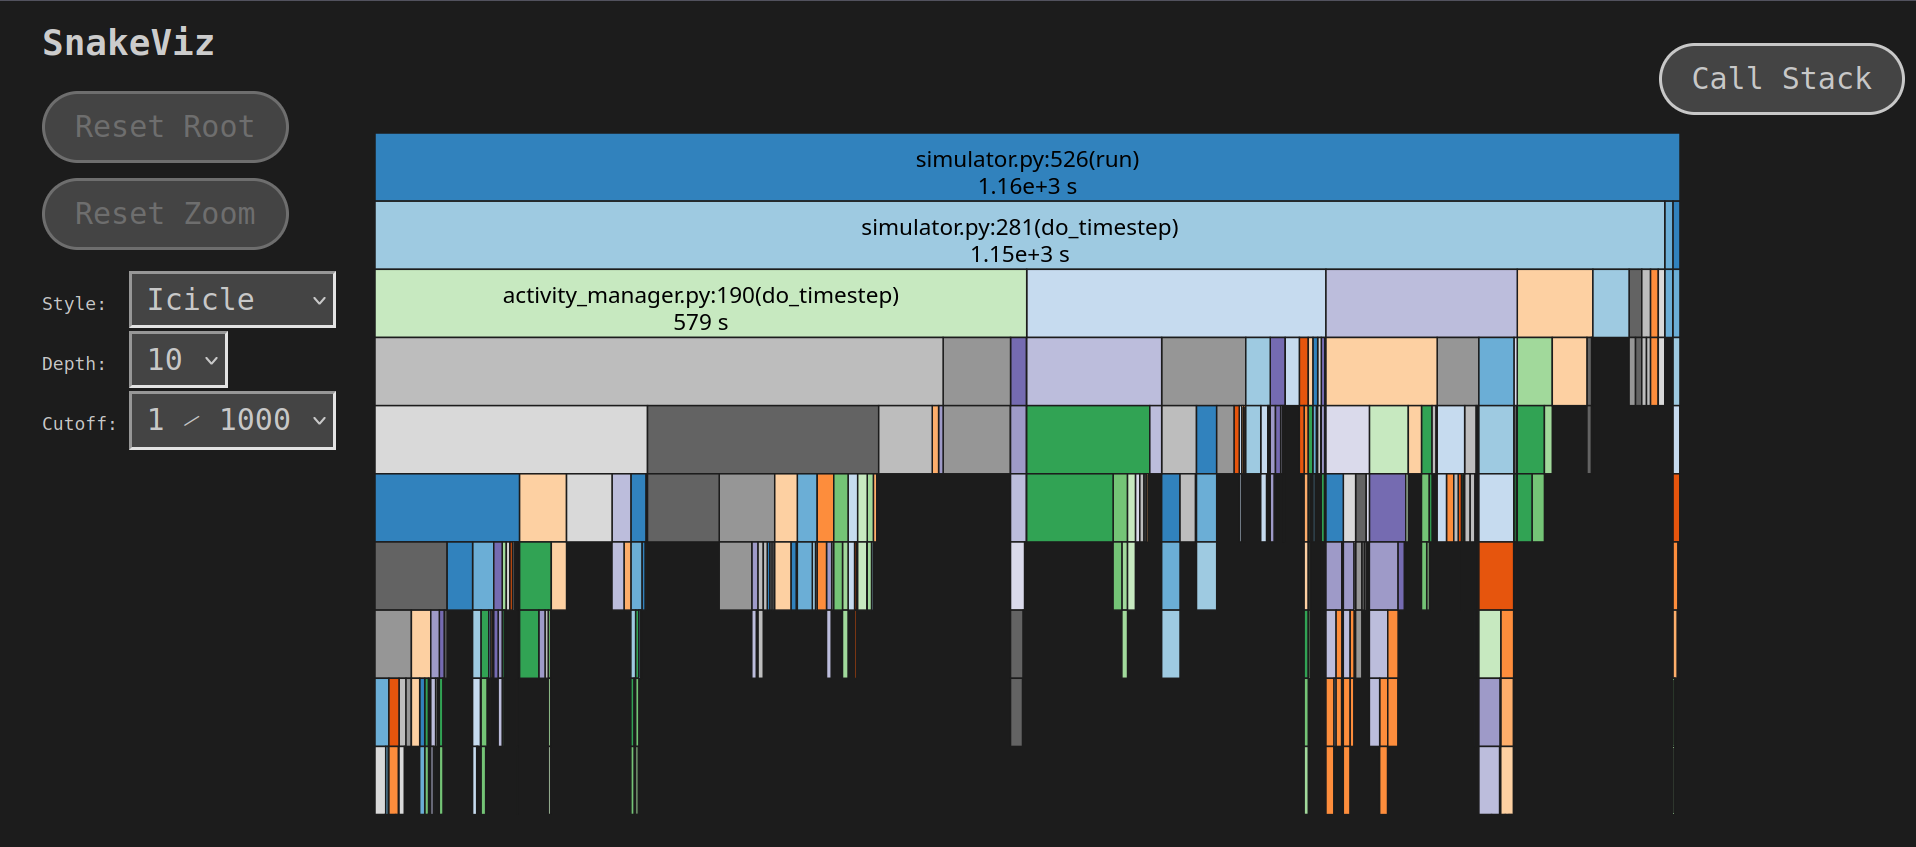
\includegraphics[width=1.0\textwidth]{images/snakeviz_june_serial.png}
    \caption{Example of the SnakeViz GUI showing the runtimes of functions and their position within the call stack.}
\end{figure}

With this serial profile, we can gain knowledge of functions which take up
considerable amounts of the runtime. The most significant portions of the
runtime sit within the highest level \verb|do_timestep| functions in \verb|simulator.py|.
This is a good sign as it implies that the majority of the runtime is within
computations rather than configuration or I/O. In order of runtime consumption
we have:
\begin{itemize}
    \item \verb|do_timesteps| in \verb|activity_manager.py| this uses up a considerable amount of
  the runtime of \verb|do_timsteps| within \verb|simulator.py|. This function is largely
calling:
    \begin{itemize}
        \item \verb|move_people_to_active_subgroups| in \verb|activity_manager.py| which in turn are
   largely made of:
        \begin{itemize}
            \item \verb|move_to_active_subgroup| in \verb|activity_manager.py| (which also is largely
    based on \verb|get_subgroup_for_person_and_housemates| in \verb|leisure.py| and then
\verb|get_leisure_subgroup| in \verb|social_venue_distributor.py|)
        \end{itemize}
        \item \verb|apply| in \verb|individual_policies.py|
    \end{itemize}
    \item \verb|time_step_for_group| in \verb|interaction.py|. This function is largely calling:
    \begin{itemize}
        \item \verb|get_interactive_group| in \verb|household.py| which in turn is largely made of:
        \begin{itemize}
            \item \verb|__init__| in \verb|interactive.py|
        \end{itemize}
        \item \verb|time_step_for_subgroup| in \verb|interaction.py| which in turn is largely calling:
        \begin{itemize}
            \item \verb|_gets_infected| in \verb|interaction.py|
            \item \verb|sum| in \verb|_methods.py|
        \end{itemize}
    \end{itemize}
    \item \verb|do_timestep| in \verb|epidemiology.py| which is largely calling
    \begin{itemize}
        \item \verb|update_health_status| in \verb|epidemiology.py| which in turn is largely calling:
        \begin{itemize}
            \item \verb|update_health_status| in \verb|infection.py|
            \item \verb|apply| in \verb|medical_care_policies.py|
        \end{itemize}
    \end{itemize}
\end{itemize}
Therefore, with these functions highlighted consuming a relatively significant
portion of runtime, we can list them as potential bottlenecks and hence as
candidates for further performance investigations. However, first it is useful
to begin to do some profiling with some parallel runs to see how the proportion
of runtime spent in the above functions varies with the number of processes.

\subsection{Parallel}
The \verb|cProfile| module can also be setup to generate profiling data for each
rank, and by comparing the outputs from \verb|snakeviz| it can be possible to get
some ideas about load imbalances. For example, on ranks that frequently idle
the icicle graph shows blank spaces where there appears to be buffering. 

This is far from ideal, and is no where near as sophisticated as truly
MPI-aware profilers and tracers such as Score-P/Scalasca, but it can push you
in the right direction.

\section{Scaling}
\begin{figure}
    \centering
    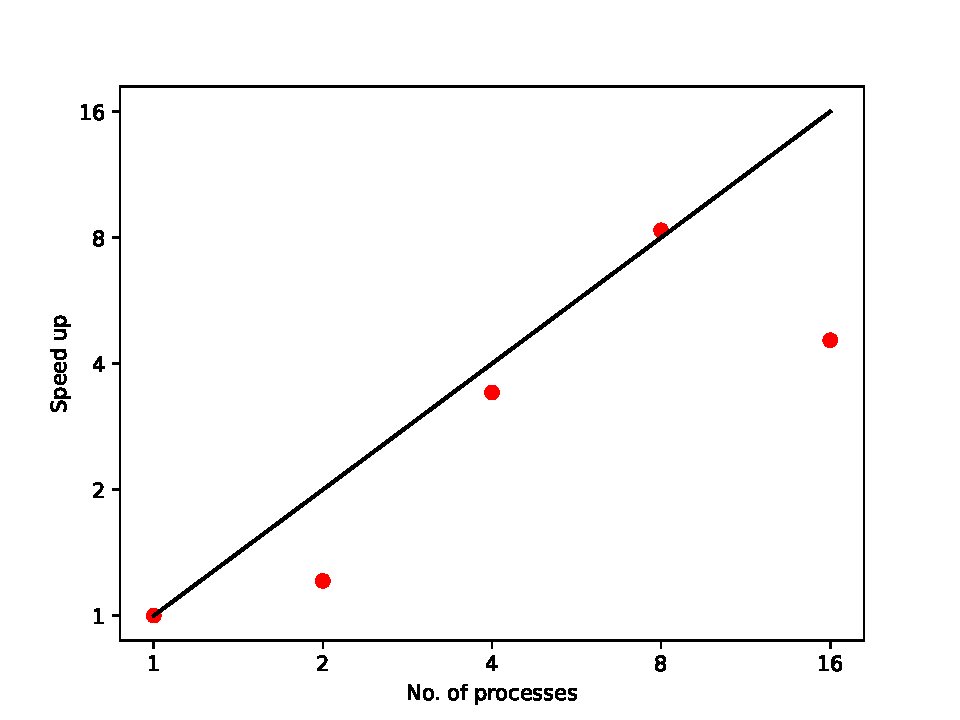
\includegraphics[width=0.75\textwidth]{images/june_lon_strong.pdf} \\
    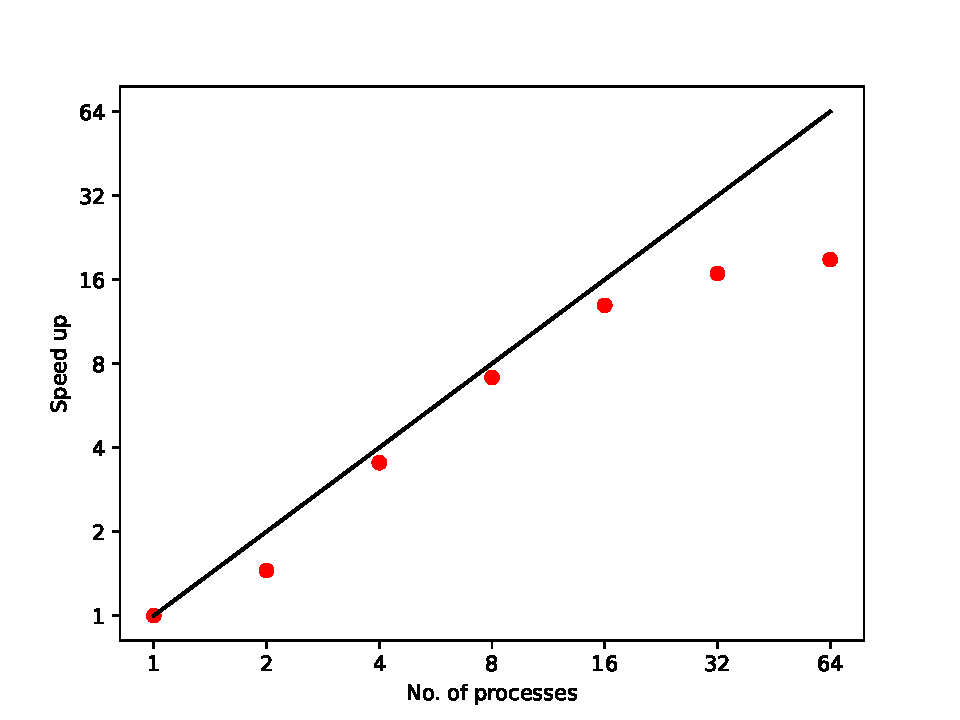
\includegraphics[width=0.75\textwidth]{images/june_eng_strong.pdf}
    \caption{Strong scaling of the full}
\end{figure}

\section{Static code analysis}
The profiling data shows some functions which occupy significant portions of
runtime and so the first task is to do a naive static code analysis, i.e.,
simply reading the code to gain a brutal first impression of performance
bottlenecks. Can we see a kernel which is consistent with this significant
runtime? Are there branching control flows within for loops that could hit
performance.

This static code analysis will always be relatively limited in it's complexity
and productivity. However, it can begin a process of the performance analyst to
'dig into' the code, i.e., to begin understanding the areas of computational
intensity.

\textbf{Checkpoint:} This provides another where there can be dialogue between the
performance analyst and the researcher, i.e., if the performance analyst has
isolated code blocks which present performance bottlenecks these can be
presented to the researcher. It seems beneficial if the analyst can provide a
brief report on these functions/kernels and any summaries, or hypotheses, they
conjure to liaise with the researcher. It may be that there are algorithmic
discussions around this performance and this can direct the performance analyst
further in the next steps after static code analysis. Building mini-apps or
proxies? Application benchmarking?

\subsection{do_timestep in activity_manager.py}
\textbf{FINDINGS}

\subsection{time_step_for_subgroup in interaction.py}
\textbf{FINDINGS}

\subsection{do_timestep in epidemiology.py}
\textbf{FINDINGS}

\section{Load balancing}
Having looked into the scaling behaviour, the code naively appears to scale
well up to approximately 16 ranks when running the London test case. However,
looking into the per rank scaling behaviour tells a different story. It appears
that some ranks are sat idle for considerable time whilst other ranks are busy
in the computation.

There are therefore two different focuses of these findings:
\begin{enumerate}
    \item There is an imbalancing of compute across ranks:
    \begin{enumerate}
        \item This could be a call pattern issue, i.e., some ranks are just
designed to carry certain parts of the compute. For example, it may be that
some components are designed to be called in serial by the 0th rank
        \item Otherwise it could be an imbalance of the data being acted on
    \end{enumerate}
    \item There could also be certain compute bottlenecks, i.e., some functions are
   showing up as occupying significant compute time simply because there are
indeed bottlenecks due to inefficient algorithmic design (rather than due to
load imbalancing)
\end{enumerate}


The idle ranks appears to indicate a load balancing issue, and my hypothesis is
that this is due to an imbalancing of the input data, i.e., I believe the
partitioning of the 'world' population is highly unequal. I have added \verb|print|
statements to the setup stage of \verb|run_simulation.py| such that each rank will
print the population size of its domain. An example of the London test case
running on 16 ranks shows:
\begin{verbatim}
mpi_rank10 has loaded domain with population 7539
mpi_rank9 has loaded domain with population 7691
mpi_rank15 has loaded domain with population 8483
mpi_rank13 has loaded domain with population 9070
mpi_rank14 has loaded domain with population 9142
mpi_rank12 has loaded domain with population 10309
mpi_rank8 has loaded domain with population 11262
mpi_rank6 has loaded domain with population 14326
mpi_rank5 has loaded domain with population 13681
mpi_rank0 has loaded domain with population 9405
mpi_rank4 has loaded domain with population 14099
mpi_rank3 has loaded domain with population 15817
mpi_rank11 has loaded domain with population 19107
mpi_rank2 has loaded domain with population 21648
mpi_rank1 has loaded domain with population 44018
mpi_rank7 has loaded domain with population 16937
\end{verbatim}
Therefore, rank 1 is operating on a population 5.84 times the size of rank 10
which is creating quite a significant load imbalance. Therefore, I think the
best course of action would be focus on redistributing the domain partitioning
across MPI ranks to satiate this imbalance. Then a further profiling can take
place on this 're-balanced' JUNE and further hotspots and bottlenecks can be
isolated. However, with the limited Python profiling currently available for
this project it would be difficult to infer much performance information beyond
this imbalance without addressing it first as it is almost impossible to know
whether certain functions are truly performance bottlenecks or are just a
symptom of this imbalance.

\section{Work overview}
In essence, our profiling work has consisted of:

1. Get the code up and running - this can be a considerable portion of work as
   the code base may have significant dependencies... (this plays into comments
around reproducibility analysis)
2. Review the workflow of the code, i.e., are certain scripts to be run first
3. Understand the parallelisation scheme - MPI, OpenMP+MPI, GPU, etc.
4. Note the test case, and how this test case relates to the 'typical'
   simulations this code is used for
5. Run a serial job in serial to understand the raw runtime and memory usage -
   again now review how this would scale to meet the requirements of a typical
'full' simulation
6. Profile!

\section{Conclusion (as of 17/04/25)}